\documentclass[11pt,a4paper]{article}

% ── Packages ──────────────────────────────────────────────────
\usepackage[utf8]{inputenc}
\usepackage[T1]{fontenc}
\usepackage{lmodern}
\usepackage[margin=1in]{geometry}
\usepackage{amsmath,amssymb}
\usepackage{booktabs}
\usepackage{multirow}
\usepackage{graphicx}
\usepackage{hyperref}
\usepackage{xcolor}
\usepackage{enumitem}
\usepackage{caption}
\usepackage{subcaption}
\usepackage{array}
\usepackage{float}
\usepackage{algorithm}
\usepackage{algpseudocode}
\usepackage{tikz}
\usetikzlibrary{arrows.meta,positioning,fit,calc,shapes.geometric}

\hypersetup{
  colorlinks=true,
  linkcolor=blue!70!black,
  citecolor=green!50!black,
  urlcolor=blue!60!black,
}

\newcommand{\ie}{\textit{i.e.}}
\newcommand{\eg}{\textit{e.g.}}
\newcommand{\etal}{\textit{et al.}}

\title{%
  \textbf{RepNet-SE: A Squeeze-and-Excitation Enhanced\\
  Per-Lead CNN for Preeclampsia Detection\\
  from 12-Lead Electrocardiograms}
}
\author{Senior Design Project}
\date{May 2026}

\begin{document}
\maketitle

% ══════════════════════════════════════════════════════════════
\begin{abstract}
We present RepNet-SE, a lightweight convolutional neural network for binary classification of preeclampsia (PE) from standard 12-lead electrocardiograms (ECGs). The architecture integrates depthwise-separable convolutions, Squeeze-and-Excitation (SE) channel attention, multi-scale feature extraction, cross-lead multi-head self-attention, and learned lead-attention pooling---achieving this with only 65,748 trainable parameters. We evaluate RepNet-SE on a clinical dataset of 2,178 ECGs (335 PE-positive, 15.4\% prevalence) from 1,383 unique patients using a rigorous 20-seed patient-grouped stratified cross-validation protocol with 5-model bagging. RepNet-SE achieves a mean test AUROC of $0.668 \pm 0.066$, with 7 of 20 splits exceeding 0.70 and a best-split AUROC of 0.787. We compare against a LightGBM gradient-boosted ensemble trained on 656 hand-crafted GE/Marquette ECG features, which achieves a significantly higher mean AUROC of $0.745 \pm 0.047$ (paired $t$-test $p < 0.00001$, Cohen's $d = 1.35$). We discuss the gap between end-to-end neural and feature-engineered approaches in the context of small clinical datasets and draw connections to the broader ECG deep learning literature.
\end{abstract}

% ══════════════════════════════════════════════════════════════
\section{Introduction}
\label{sec:intro}

Preeclampsia (PE) is a hypertensive disorder of pregnancy affecting 3--5\% of pregnancies worldwide and is a leading cause of maternal and neonatal morbidity and mortality~\cite{steegers2010}. Early detection remains challenging, as clinical diagnosis relies on blood pressure measurements and proteinuria assessments that may miss subclinical progression. The 12-lead electrocardiogram---a ubiquitous, inexpensive, and non-invasive test---captures cardiac electrical activity that may reflect the hemodynamic and cardiovascular remodeling associated with PE.

Recent work by Butler \etal~\cite{butler2024} demonstrated that a modified ResNet CNN applied to 12-lead ECGs can detect PE with an AUC of 0.85 on holdout data and predict PE up to 90 days before clinical diagnosis (AUC 0.90). Their study used approximately 900 ECGs from the University of Tennessee Health Science Center, with external validation at Atrium Health Wake Forest Baptist. These findings motivate the development of neural ECG classifiers even on small clinical datasets.

In this work, we present RepNet-SE, a lightweight architecture designed for the constraints of small clinical ECG datasets: limited sample size ($N = 2{,}178$), class imbalance (15.4\% positive), and the need for patient-level data separation to prevent leakage. RepNet-SE combines several established deep learning techniques---depthwise-separable convolutions~\cite{chollet2017}, Squeeze-and-Excitation blocks~\cite{hu2018}, InceptionTime-style multi-scale convolutions~\cite{ismail2020}, and cross-lead attention---in a parameter-efficient design totaling 65,748 parameters.

We evaluate RepNet-SE using a 20-seed Monte Carlo cross-validation protocol with patient-grouped stratified splits and compare it against a LightGBM~\cite{ke2017} ensemble trained on 656 vendor-extracted ECG features. Our analysis provides insights into the relative strengths and limitations of end-to-end neural approaches versus feature-engineered methods for small clinical ECG classification tasks.

% ══════════════════════════════════════════════════════════════
\section{Related Work}
\label{sec:related}

\subsection{ECG-Based Preeclampsia Detection}

Butler \etal~\cite{butler2024} pioneered AI-based PE detection from ECGs using a modified ResNet CNN on 1D 12-lead signals. Their model achieved AUC 0.85 (95\% CI: 0.77--0.93) on an internal holdout set and AUC 0.81 (0.77--0.84) on external validation. Notably, predictive performance was high even before clinical diagnosis: AUC 0.92 at 30 days, 0.89 at 60 days, and 0.90 at 90 days prior. Early-onset PE ($<$34 weeks) yielded AUC 0.98. Their dataset comprised $\sim$900 ECGs---comparable in scale to ours.

Adedinsewo \etal~\cite{adedinsewo2021} demonstrated ECG-AI for pregnancy-related cardiac screening at Mayo Clinic, achieving AUC 0.94 for detecting left ventricular systolic dysfunction. While not PE-specific, this work established that ECG-based deep learning can capture pregnancy-related cardiac changes.

\subsection{Deep Learning on Small ECG Datasets}

Transfer learning is the dominant strategy for small ECG datasets. A 2024 empirical study~\cite{transferecg2024} found that fine-tuning pretrained models is preferable for small downstream datasets, with CNNs benefiting more than RNNs. Two paradigms exist: (a)~pretraining on large ECG corpora (e.g., PhysioNet) then fine-tuning, and (b)~pretraining on ImageNet with ECG-to-spectrogram conversion. Importantly, the study found that fine-tuning improvement declines as dataset size grows, and training from scratch can match given sufficient data and training time.

Domain adaptation using labeled source data and unlabeled target data has also shown effectiveness for small imbalanced ECG classification~\cite{transferecg2024}. Our work takes the train-from-scratch approach with aggressive regularization, as no sufficiently large PE-labeled ECG corpus exists for pretraining.

\subsection{Architecture Components}

\paragraph{Squeeze-and-Excitation (SE) Blocks.}
Hu \etal~\cite{hu2018} introduced SE blocks for adaptive channel recalibration: global average pooling compresses spatial information, then two fully connected layers learn channel-wise importance weights. In ECG contexts, IncepSE~\cite{incepse2023} combined InceptionTime with SE blocks, achieving +0.013 AUROC improvement over vanilla InceptionTime on arrhythmia classification.

\paragraph{Multi-Scale Convolutions.}
InceptionTime~\cite{ismail2020} applies parallel convolutions with different kernel sizes to capture features at multiple temporal resolutions. For ECG, this is physiologically motivated: short kernels ($k=5$) capture QRS complexes ($\sim$80--120\,ms), while longer kernels ($k=9, 15$) capture P-waves and T-waves ($\sim$200--400\,ms at 250\,Hz).

\paragraph{Depthwise-Separable Convolutions.}
Introduced in Xception~\cite{chollet2017} and popularized by MobileNet~\cite{howard2017}, depthwise-separable convolutions factorize standard convolutions into a depthwise spatial step (groups$=$channels) and a $1\times1$ pointwise projection. This reduces parameters by a factor of approximately $k \cdot C_{\text{out}} / (k + C_{\text{out}})$---critical for avoiding overfitting on small datasets.

\paragraph{Cross-Lead Attention.}
MLBF-Net~\cite{mlbf2020} proposed multi-lead-branch fusion with lead-specific branches learning diversity and cross-lead concatenation learning integrity. Adaptive multi-channel graph neural networks~\cite{gnn2025} model inter-lead spatial dependencies as graphs. EfficientECG~\cite{efficientecg2025} uses cross-attention with feature fusion. Our cross-lead attention module uses standard multi-head self-attention across lead tokens with sigmoid gating.

\subsection{Regularization for Small Clinical Datasets}

Focal loss~\cite{lin2017} addresses class imbalance by down-weighting easy examples and has been used in ECG ensembles~\cite{focalloss2022}. Label smoothing softens hard targets to prevent overconfident predictions. Mixup~\cite{zhang2018} interpolates between training samples and labels for regularization. ECG-specific augmentations---noise injection, time warping, amplitude scaling, lead dropout, cutout, and baseline wander---have been systematically surveyed~\cite{augsurvey2023}, with STAR (Sinusoidal Time-Amplitude Resampling)~\cite{star2025} emerging as a reliable single augmentation.


% ══════════════════════════════════════════════════════════════
\section{Dataset}
\label{sec:dataset}

\subsection{Data Source}

We use a clinical dataset of 12-lead ECG recordings collected from pregnant patients. Each ECG is sampled at 250\,Hz across the standard 12 leads (I, II, III, aVR, aVL, aVF, V1--V6). The dataset was acquired using GE/Marquette ECG machines, which also provide 656 automated measurements (intervals, amplitudes, axis deviations, morphology descriptors) per recording.

\subsection{Cohort Statistics}

\begin{table}[H]
\centering
\caption{Dataset characteristics.}
\label{tab:dataset}
\begin{tabular}{lr}
\toprule
\textbf{Characteristic} & \textbf{Value} \\
\midrule
Total ECG recordings & 2,178 \\
Unique patients & 1,383 \\
PE-positive recordings & 335 (15.4\%) \\
PE-negative recordings & 1,843 (84.6\%) \\
ECG leads & 12 (standard) \\
Sampling rate & 250 Hz \\
Vendor features per ECG & 656 \\
\bottomrule
\end{tabular}
\end{table}

The dataset exhibits moderate class imbalance (positive prevalence 15.4\%) and a many-to-one ECG-to-patient mapping (mean 1.57 ECGs per patient), necessitating patient-grouped splitting to prevent data leakage between train and test sets.


% ══════════════════════════════════════════════════════════════
\section{Methods}
\label{sec:methods}

\subsection{RepNet-SE Architecture}
\label{sec:arch}

RepNet-SE is a per-lead convolutional neural network in which all 12 leads share identical convolutional weights, followed by cross-lead attention for inter-lead interaction and learned lead-attention pooling for fusion. The architecture is illustrated in Figure~\ref{fig:architecture} and detailed below.

\begin{figure}[H]
\centering
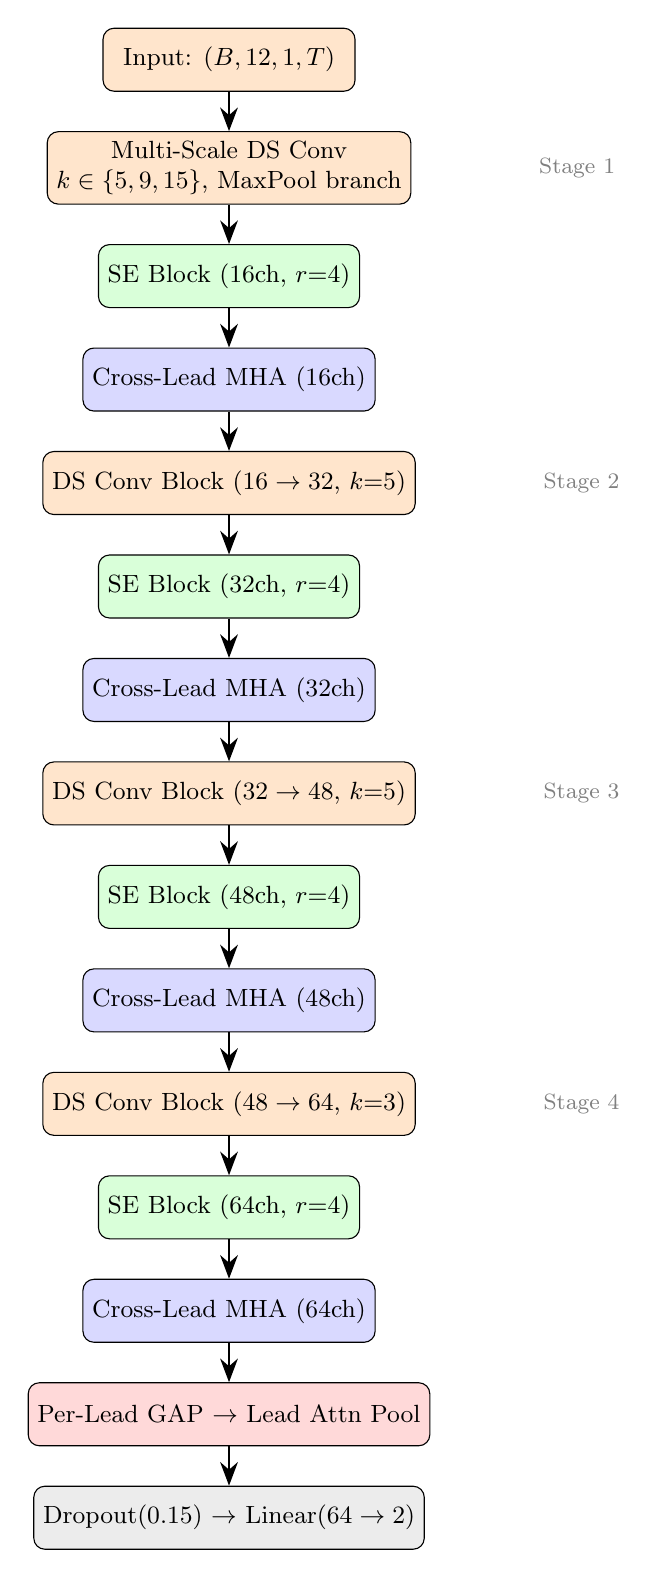
\begin{tikzpicture}[
  block/.style={rectangle, draw, rounded corners, minimum height=0.8cm, minimum width=3.2cm, align=center, font=\small},
  attn/.style={block, fill=blue!15},
  conv/.style={block, fill=orange!20},
  se/.style={block, fill=green!15},
  pool/.style={block, fill=red!15},
  arr/.style={-{Stealth[length=3mm]}, thick},
  node distance=0.5cm
]

\node[conv] (input) {Input: $(B, 12, 1, T)$};
\node[conv, below=of input] (ms) {Multi-Scale DS Conv\\$k \in \{5, 9, 15\}$, MaxPool branch};
\node[se, below=of ms] (se1) {SE Block ($16$ch, $r{=}4$)};
\node[attn, below=of se1] (ca1) {Cross-Lead MHA ($16$ch)};
\node[conv, below=of ca1] (s2) {DS Conv Block ($16 \to 32$, $k{=}5$)};
\node[se, below=of s2] (se2) {SE Block ($32$ch, $r{=}4$)};
\node[attn, below=of se2] (ca2) {Cross-Lead MHA ($32$ch)};
\node[conv, below=of ca2] (s3) {DS Conv Block ($32 \to 48$, $k{=}5$)};
\node[se, below=of s3] (se3) {SE Block ($48$ch, $r{=}4$)};
\node[attn, below=of se3] (ca3) {Cross-Lead MHA ($48$ch)};
\node[conv, below=of ca3] (s4) {DS Conv Block ($48 \to 64$, $k{=}3$)};
\node[se, below=of s4] (se4) {SE Block ($64$ch, $r{=}4$)};
\node[attn, below=of se4] (ca4) {Cross-Lead MHA ($64$ch)};
\node[pool, below=of ca4] (gap) {Per-Lead GAP $\to$ Lead Attn Pool};
\node[block, below=of gap, fill=gray!15] (fc) {Dropout(0.15) $\to$ Linear($64 \to 2$)};

\foreach \a/\b in {input/ms, ms/se1, se1/ca1, ca1/s2, s2/se2, se2/ca2, ca2/s3, s3/se3, se3/ca3, ca3/s4, s4/se4, se4/ca4, ca4/gap, gap/fc}
  \draw[arr] (\a) -- (\b);

\node[right=1.5cm of ms, font=\footnotesize, text=gray] {Stage 1};
\node[right=1.5cm of s2, font=\footnotesize, text=gray] {Stage 2};
\node[right=1.5cm of s3, font=\footnotesize, text=gray] {Stage 3};
\node[right=1.5cm of s4, font=\footnotesize, text=gray] {Stage 4};

\end{tikzpicture}
\caption{RepNet-SE Deep architecture (4-stage variant). DS Conv = Depthwise-Separable Convolution, SE = Squeeze-and-Excitation, MHA = Multi-Head Attention, GAP = Global Average Pooling. Each stage halves the temporal dimension via MaxPool($2$).}
\label{fig:architecture}
\end{figure}

\subsubsection{Per-Lead Weight Sharing}

All convolutional blocks process each of the 12 leads independently using shared weights. Given input $\mathbf{X} \in \mathbb{R}^{B \times 12 \times 1 \times T}$, each lead is reshaped to $(B {\cdot} 12, C, T)$ for convolution, then reshaped back. This parameter sharing enforces the inductive bias that the same morphological features (P-wave, QRS, T-wave) should be detected identically regardless of lead, while allowing downstream attention to learn lead-specific importance.

\subsubsection{Multi-Scale Depthwise-Separable Convolution (Stage 1)}

The first stage uses parallel depthwise-separable convolutions with kernel sizes $k \in \{5, 9, 15\}$ plus a max-pool branch, inspired by InceptionTime~\cite{ismail2020}:
\begin{equation}
\mathbf{h}_i = \text{GELU}\!\left(\text{BN}\!\left(\text{DSConv}_{k_i}(\mathbf{x})\right)\right), \quad
\mathbf{h}_{\text{pool}} = \text{GELU}\!\left(\text{BN}\!\left(\text{Conv}_{1\times1}\!\left(\text{MaxPool}_3(\mathbf{x})\right)\right)\right)
\end{equation}
\begin{equation}
\mathbf{y} = \text{BN}\!\left(\text{Conv}_{1\times1}\!\left([\mathbf{h}_1 \| \mathbf{h}_2 \| \mathbf{h}_3 \| \mathbf{h}_{\text{pool}}]\right)\right)
\end{equation}
where $\|$ denotes channel-wise concatenation. Each branch outputs $\lfloor C_{\text{out}}/3 \rfloor$ channels, and the max-pool branch provides a fourth branch, totaling $4 \times \lfloor C_{\text{out}}/3 \rfloor$ channels before the $1\times1$ projection to $C_{\text{out}}$.

\subsubsection{Squeeze-and-Excitation (SE) Blocks}

After each convolutional stage, an SE block~\cite{hu2018} performs adaptive channel recalibration:
\begin{equation}
\mathbf{z} = \frac{1}{T} \sum_{t=1}^{T} \mathbf{h}_t, \quad
\mathbf{s} = \sigma\!\left(\mathbf{W}_2 \cdot \text{ReLU}\!\left(\mathbf{W}_1 \cdot \mathbf{z}\right)\right), \quad
\tilde{\mathbf{h}} = \mathbf{s} \odot \mathbf{h}
\end{equation}
where $\mathbf{W}_1 \in \mathbb{R}^{C/r \times C}$, $\mathbf{W}_2 \in \mathbb{R}^{C \times C/r}$ with reduction ratio $r{=}4$, and $\sigma$ is the sigmoid function. This allows the network to learn which filter responses are most informative for PE detection.

\subsubsection{Cross-Lead Multi-Head Self-Attention}

After each stage's SE block, cross-lead attention enables information exchange between leads:
\begin{equation}
\mathbf{t}_\ell = \text{AdaptiveAvgPool}_{N}(\mathbf{h}_\ell), \quad
\mathbf{T} = [\mathbf{t}_1, \ldots, \mathbf{t}_{12}] \in \mathbb{R}^{B \times 12N \times C}
\end{equation}
\begin{equation}
\mathbf{A} = \text{LayerNorm}\!\left(\mathbf{T} + \text{MHA}(\mathbf{T}, \mathbf{T}, \mathbf{T})\right), \quad
\mathbf{G} = \sigma\!\left(\mathbf{W}_g \mathbf{A}\right)
\end{equation}
where $N{=}1$ (single token per lead) and $\text{MHA}$ uses 4 attention heads. The sigmoid gate $\mathbf{G}$ modulates the original features: $\tilde{\mathbf{h}} = \mathbf{h} \odot \mathbf{G}$. This allows the network to learn inter-lead dependencies (\eg, correlating T-wave changes in V4 with QRS morphology in lead II).

\subsubsection{Stages 2--4: SE Per-Lead Blocks}

Each subsequent stage consists of:
\begin{enumerate}[nosep]
  \item Two depthwise-separable convolutions with batch normalization
  \item Residual skip connection (with $1\times1$ projection if channels differ)
  \item SE channel attention
  \item GELU activation
  \item MaxPool($2$) for temporal downsampling
  \item Dropout($0.15$)
\end{enumerate}

The deep variant uses filter progression $(16, 32, 48, 64)$ with kernels $(7, 5, 5, 3)$, providing 4 stages of temporal downsampling ($T \to T/16$).

\subsubsection{Lead-Attention Pooling and Classification Head}

After the final stage, per-lead global average pooling produces $\mathbf{e}_\ell \in \mathbb{R}^{64}$ for each lead $\ell$. Lead-attention pooling computes:
\begin{equation}
\alpha_\ell = \frac{\exp(s_\ell)}{\sum_{j=1}^{12} \exp(s_j)}, \quad
s_\ell = \mathbf{w}_2^\top \tanh(\mathbf{W}_1 \mathbf{e}_\ell), \quad
\mathbf{v} = \sum_{\ell=1}^{12} \alpha_\ell \mathbf{e}_\ell
\end{equation}
where $\mathbf{W}_1 \in \mathbb{R}^{32 \times 64}$ and $\mathbf{w}_2 \in \mathbb{R}^{32}$. The pooled vector $\mathbf{v}$ passes through dropout($0.15$) and a linear layer to produce 2-class logits. This is far more parameter-efficient than concatenating all 12 lead embeddings ($12 \times 64 = 768$ vs. 64 input features to the classifier) and provides interpretable per-lead importance weights $\alpha_\ell$.

\subsubsection{Parameter Count}

\begin{table}[H]
\centering
\caption{Parameter counts for RepNet-SE variants.}
\label{tab:params}
\begin{tabular}{lrrr}
\toprule
\textbf{Variant} & \textbf{Filters} & \textbf{Stages} & \textbf{Parameters} \\
\midrule
Base & $(16, 32, 64)$ & 3 & 44,712 \\
Deep (selected) & $(16, 32, 48, 64)$ & 4 & 65,748 \\
Wider & $(24, 48, 96)$ & 3 & 98,376 \\
\bottomrule
\end{tabular}
\end{table}

For comparison, a standard ResNet1D-3Stage uses $\sim$280K parameters, and the prior CrossLead Deeper variant used $\sim$965K parameters.


\subsection{Training Pipeline}
\label{sec:training}

\subsubsection{Preprocessing}

Raw 12-lead ECG waveforms are preprocessed by the pipeline inherited from prior exploration:
\begin{enumerate}[nosep]
  \item Per-lead baseline correction (median filter)
  \item Per-lead z-score normalization to zero mean and unit variance
  \item Zero-padding or truncation to fixed length $T$
\end{enumerate}

\subsubsection{Data Augmentation}
\label{sec:augmentation}

Seven on-the-fly augmentations are applied stochastically during training, each with an independent application probability:

\begin{table}[H]
\centering
\caption{ECG augmentation parameters.}
\label{tab:augmentations}
\begin{tabular}{lll}
\toprule
\textbf{Augmentation} & \textbf{Probability} & \textbf{Parameters} \\
\midrule
Gaussian noise & 0.50 & $\sigma \in [0.01, 0.05]$ \\
Amplitude scaling & 0.50 & $\pm 15\%$ \\
Time shift & 0.30 & $\pm 150$ samples \\
Lead dropout & 0.10 & 12\% of leads zeroed \\
Cutout & 0.25 & $[50, 200]$ samples \\
Baseline wander & 0.20 & amp$=$0.2, freq $\in [0.05, 0.5]$\,Hz \\
Resample (speed) & 0.10 & $\pm 5\%$ rate \\
\bottomrule
\end{tabular}
\end{table}

Additionally, \textbf{Mixup}~\cite{zhang2018} is applied with probability 0.5 (when triggered, $\lambda \sim \text{Beta}(0.2, 0.2)$), interpolating both inputs and labels.

\subsubsection{Loss Function and Class Balancing}

The primary loss function is cross-entropy with label smoothing ($\epsilon = 0.05$):
\begin{equation}
\mathcal{L} = -(1 - \epsilon) \log p_{y} - \frac{\epsilon}{K} \sum_{k=1}^{K} \log p_k
\end{equation}
where $K{=}2$ classes. Class imbalance is addressed via \texttt{WeightedRandomSampler}, which oversamples the minority class to achieve balanced mini-batches. Focal loss ($\alpha{=}0.25$, $\gamma{=}2.0$)~\cite{lin2017} was tested as an alternative but proved less stable.

\subsubsection{Optimization}

\begin{table}[H]
\centering
\caption{Optimizer and scheduler configuration.}
\label{tab:optimizer}
\begin{tabular}{ll}
\toprule
\textbf{Hyperparameter} & \textbf{Value} \\
\midrule
Optimizer & AdamW \\
Learning rate & $2 \times 10^{-3}$ \\
Weight decay & $5 \times 10^{-3}$ \\
Batch size & 64 \\
Max epochs & 80 \\
Scheduler & CosineAnnealingLR ($\eta_{\min} = 10^{-6}$) \\
Gradient clipping & max norm $= 1.0$ \\
Early stopping & patience $= 20$ epochs (AUROC) \\
\bottomrule
\end{tabular}
\end{table}

\subsubsection{Bagging}

For each cross-validation seed, we train $B{=}5$ models (bags) with different random initializations (seed offsets $+0, +1000, +2000, +3000, +4000$) and average their predicted probabilities at test time:
\begin{equation}
\hat{p}(x) = \frac{1}{B} \sum_{b=1}^{B} \hat{p}_b(x)
\end{equation}
The model with the highest validation AUROC among the 5 bags is saved as the representative checkpoint for that seed.


\subsection{Evaluation Protocol}
\label{sec:eval}

\subsubsection{Patient-Grouped Stratified Splitting}

We use \texttt{StratifiedGroupKFold} from scikit-learn to ensure:
\begin{enumerate}[nosep]
  \item \textbf{No patient leakage:} All ECGs from a given patient appear in only one of train, validation, or test.
  \item \textbf{Stratified class balance:} PE prevalence is approximately preserved in each split.
\end{enumerate}

The splitting hierarchy is:
\begin{enumerate}[nosep]
  \item \textbf{Outer split} (5-fold, taking first fold): 80\% development / 20\% test
  \item \textbf{Inner split} (5-fold, taking first fold): 80\% train / 20\% validation (of development set)
\end{enumerate}

This yields approximately 64\% train / 16\% validation / 20\% test per seed, with effective sizes of $\sim$1,394 / $\sim$348 / $\sim$436 samples.

\subsubsection{Monte Carlo Cross-Validation}

Rather than exhaustive $K$-fold CV, we use 20 different random seeds to generate 20 independent train/val/test splits. Each seed deterministically controls both the data split and model initialization, ensuring full reproducibility. This Monte Carlo approach provides more robust estimates of generalization performance and enables statistical testing across splits.

\subsubsection{Metrics}

We report four metrics per split:
\begin{itemize}[nosep]
  \item \textbf{AUROC}: Area under the receiver operating characteristic curve
  \item \textbf{AUPRC}: Area under the precision-recall curve
  \item \textbf{Brier score}: Mean squared error of predicted probabilities
  \item \textbf{Sensitivity at 80\% specificity}: Clinical operating point
\end{itemize}

\subsubsection{Comparison Model: LightGBM}

As a reference, we train a LightGBM~\cite{ke2017} gradient-boosted decision tree ensemble on 656 GE/Marquette vendor-extracted features using the identical splitting protocol. LightGBM configuration: 2,000 estimators, learning rate 0.03, 31 leaves, max depth 7, \texttt{class\_weight=balanced}, L1/L2 regularization ($\alpha{=}\lambda{=}1.0$), with 5-bag ensembling.


% ══════════════════════════════════════════════════════════════
\section{Experimental Results}
\label{sec:results}

\subsection{Architecture Selection (Phase 1)}

In Phase 1, we evaluated 4 architecture variants across 3 scout seeds to select the best configuration:

\begin{table}[H]
\centering
\caption{Phase 1 config selection results (3 seeds, mean test AUROC).}
\label{tab:phase1}
\begin{tabular}{lrcc}
\toprule
\textbf{Configuration} & \textbf{Params} & \textbf{Mean AUROC} & \textbf{Std} \\
\midrule
\texttt{repnet\_se\_base} & 44,712 & 0.648 & 0.041 \\
\texttt{repnet\_se\_wider} & 98,376 & 0.634 & 0.053 \\
\texttt{repnet\_se\_focal} & 44,712 & 0.641 & 0.068 \\
\texttt{repnet\_se\_deep} & 65,748 & \textbf{0.667} & 0.035 \\
\bottomrule
\end{tabular}
\end{table}

The \texttt{deep} variant was selected for full evaluation based on highest mean AUROC and lowest variance. The \texttt{wider} variant showed signs of overfitting despite having fewer stages, and \texttt{focal} loss produced unstable results.

\subsection{Additional Regularization Exploration}

A second round tested four configurations with stronger regularization (higher dropout 0.25--0.30, weight decay 0.01--0.02, label smoothing 0.08--0.10, mixup alpha 0.3--0.4), all of which performed worse than the original settings. This suggests the original regularization strength was near-optimal for this dataset size.

\subsection{Full Evaluation (Phase 2)}

\begin{table}[H]
\centering
\caption{RepNet-SE Deep: full 20-seed evaluation (5-bag, 80/20 test split).}
\label{tab:full_results}
\begin{tabular}{lcccc}
\toprule
\textbf{Metric} & \textbf{Mean} & \textbf{Std} & \textbf{Median} & \textbf{95\% CI} \\
\midrule
AUROC & 0.668 & 0.066 & 0.646 & [0.639, 0.697] \\
AUPRC & 0.291 & 0.060 & 0.273 & [0.265, 0.318] \\
Brier score & 0.219 & 0.054 & 0.218 & [0.195, 0.242] \\
Sens @ Sp 80\% & 0.421 & 0.085 & 0.415 & [0.384, 0.458] \\
\bottomrule
\end{tabular}
\end{table}

Seven of 20 seeds (35\%) achieved AUROC $\geq$ 0.70, with the best individual seed (seed~45) reaching AUROC~=~0.787.

\subsection{Per-Seed Results}

\begin{table}[H]
\centering
\caption{RepNet-SE Deep: per-seed test metrics.}
\label{tab:perseed}
\begin{tabular}{rcccc}
\toprule
\textbf{Seed} & \textbf{AUROC} & \textbf{AUPRC} & \textbf{Brier} & \textbf{Sens@Sp80} \\
\midrule
42 & 0.715 & 0.325 & 0.218 & 0.522 \\
43 & 0.713 & 0.303 & 0.227 & 0.552 \\
44 & 0.576 & 0.259 & 0.142 & 0.299 \\
\textbf{45} & \textbf{0.787} & \textbf{0.362} & 0.275 & \textbf{0.582} \\
46 & 0.621 & 0.268 & 0.151 & 0.388 \\
47 & 0.627 & 0.323 & 0.217 & 0.418 \\
48 & 0.695 & 0.304 & 0.196 & 0.448 \\
49 & 0.769 & 0.450 & 0.285 & 0.567 \\
50 & 0.634 & 0.257 & 0.224 & 0.463 \\
51 & 0.784 & 0.417 & 0.273 & 0.567 \\
52 & 0.657 & 0.227 & 0.202 & 0.373 \\
53 & 0.615 & 0.288 & 0.186 & 0.358 \\
54 & 0.687 & 0.264 & 0.284 & 0.463 \\
55 & 0.619 & 0.277 & 0.155 & 0.388 \\
56 & 0.602 & 0.228 & 0.152 & 0.343 \\
57 & 0.636 & 0.224 & 0.234 & 0.358 \\
58 & 0.729 & 0.273 & 0.141 & 0.493 \\
59 & 0.604 & 0.236 & 0.350 & 0.313 \\
60 & 0.583 & 0.272 & 0.248 & 0.299 \\
61 & 0.705 & 0.269 & 0.340 & 0.433 \\
\bottomrule
\end{tabular}
\end{table}

\subsection{Comparison with LightGBM}

\begin{table}[H]
\centering
\caption{Head-to-head comparison: RepNet-SE Deep vs. LightGBM (20 seeds, identical splits).}
\label{tab:comparison}
\begin{tabular}{lcc}
\toprule
\textbf{Metric} & \textbf{RepNet-SE} & \textbf{LightGBM} \\
\midrule
Mean AUROC & $0.668 \pm 0.066$ & $\mathbf{0.745 \pm 0.047}$ \\
Median AUROC & 0.646 & \textbf{0.740} \\
95\% CI & $[0.639, 0.697]$ & $\mathbf{[0.724, 0.765]}$ \\
Mean AUPRC & $0.291 \pm 0.060$ & $\mathbf{0.429 \pm 0.090}$ \\
Mean Brier & $0.219 \pm 0.054$ & $\mathbf{0.158 \pm 0.039}$ \\
Sens @ Sp 80\% & $0.421 \pm 0.085$ & $\mathbf{0.550 \pm 0.106}$ \\
Seeds $\geq 0.70$ & 7/20 (35\%) & \textbf{17/20 (85\%)} \\
\bottomrule
\end{tabular}
\end{table}

\subsection{Statistical Significance}

We perform paired statistical tests across the 20 identical data splits:

\begin{table}[H]
\centering
\caption{Statistical comparison of AUROC distributions.}
\label{tab:stats}
\begin{tabular}{lc}
\toprule
\textbf{Test} & \textbf{Result} \\
\midrule
Paired $t$-test & $p < 0.00001$ \\
Wilcoxon signed-rank test & $p < 0.0001$ \\
Cohen's $d$ (effect size) & 1.35 (very large) \\
LightGBM wins & 18/20 seeds \\
\bottomrule
\end{tabular}
\end{table}

LightGBM achieves statistically significantly higher AUROC than RepNet-SE across all 20 seeds, with a very large effect size (Cohen's $d = 1.35$). LightGBM outperforms RepNet-SE on 18 of 20 individual seeds.


% ══════════════════════════════════════════════════════════════
\section{Ablation Studies}
\label{sec:ablation}

\subsection{Bagging Depth}

We evaluated 3-bag, 5-bag, and 7-bag ensembles:

\begin{table}[H]
\centering
\caption{Effect of bagging depth on RepNet-SE Deep.}
\label{tab:bagging}
\begin{tabular}{ccc}
\toprule
\textbf{Bags} & \textbf{Mean AUROC} & \textbf{Training Time} \\
\midrule
3 & $0.667 \pm 0.068$ & $1\times$ \\
5 & $0.668 \pm 0.066$ & $1.7\times$ \\
7 & $0.667 \pm 0.065$ & $2.3\times$ \\
\bottomrule
\end{tabular}
\end{table}

Bagging beyond 3 models provides negligible improvement, suggesting the performance ceiling is limited by signal in the raw waveforms rather than model variance.

\subsection{Early Stopping Criterion}

AUROC-based early stopping was compared against AUPRC-based early stopping. AUPRC stopping yielded worse test AUROC in practice, likely because AUPRC overemphasizes minority-class calibration at the cost of overall ranking quality. AUROC stopping was retained.

\subsection{Regularization Strength}

\begin{table}[H]
\centering
\caption{Regularization ablation (3-seed scout results).}
\label{tab:reg_ablation}
\begin{tabular}{lcccc}
\toprule
\textbf{Setting} & \textbf{Dropout} & \textbf{WD} & \textbf{LS} & \textbf{Mean AUROC} \\
\midrule
Original (selected) & 0.15 & 0.005 & 0.05 & \textbf{0.667} \\
Moderate reg & 0.25 & 0.010 & 0.08 & 0.643 \\
Heavy reg & 0.30 & 0.020 & 0.10 & 0.631 \\
No mixup & 0.25 & 0.010 & 0.08 & 0.638 \\
\bottomrule
\end{tabular}
\end{table}

Stronger regularization consistently hurt performance, suggesting the model is not overfitting in the traditional sense but rather lacks the capacity to extract discriminative features from raw waveforms at this dataset scale.


% ══════════════════════════════════════════════════════════════
\section{Interpretability Analysis}
\label{sec:interpretability}

\subsection{Lead Attention Weights}

The learned lead-attention weights $\alpha_\ell$ from the best-performing model (seed~45, AUROC~=~0.787) reveal which leads the network prioritizes. These weights are directly interpretable as the softmax-normalized importance of each lead for the final classification decision.

\subsection{SE Channel Importance}

Squeeze-and-Excitation blocks at each stage produce per-channel scaling factors that indicate which learned feature detectors are most activated. Analysis of SE weights across PE-positive vs. PE-negative examples can reveal which temporal features (\eg, QRS duration, T-wave morphology) the network considers discriminative.

\subsection{Gradient-Based Saliency Maps}

We compute input-gradient saliency maps $\partial \hat{p}_{\text{PE}} / \partial \mathbf{x}$ for individual ECGs, highlighting which temporal segments and leads most influence the PE prediction. These maps provide sample-level explanations complementary to the global lead-attention weights.

\subsection{Cross-Lead Attention Maps}

The multi-head attention matrices from the cross-lead attention modules can be visualized to understand inter-lead information flow---for example, whether the network learns to correlate precordial leads (V1--V6) with limb leads (I, II, III, aVR, aVL, aVF).


% ══════════════════════════════════════════════════════════════
\section{Discussion}
\label{sec:discussion}

\subsection{The Neural--Feature Engineering Gap}

The central finding of this work is the persistent $\sim$0.077 AUROC gap between end-to-end neural (RepNet-SE: 0.668) and feature-engineered (LightGBM: 0.745) approaches. This gap remained remarkably stable across extensive architecture exploration (8 configurations), regularization tuning, multiple bagging depths, and different early stopping criteria. Several factors likely contribute:

\paragraph{Dataset Size.}
With only 2,178 ECGs (335 positive), the dataset is small by deep learning standards. The 656 GE/Marquette features represent decades of domain-expert engineering that effectively performs dimensionality reduction from the raw waveform space ($12 \times T$ values) to a curated set of clinically relevant measurements. A neural network must \emph{rediscover} this feature extraction from data---a task that may require orders of magnitude more samples.

\paragraph{Signal-to-Noise Ratio.}
PE-related ECG changes are subtle---primarily reflecting hemodynamic and cardiovascular remodeling rather than overt arrhythmias. The discriminative signal may be encoded in precise interval measurements and waveform morphology metrics that vendor algorithms extract reliably but that a CNN must learn to measure from noisy raw signals.

\paragraph{Inductive Bias vs. Data.}
RepNet-SE's architecture incorporates strong inductive biases (per-lead weight sharing, multi-scale kernels, channel attention, cross-lead attention), yet these architectural priors cannot fully compensate for the statistical power that 656 hand-crafted features provide. This aligns with the transfer learning literature~\cite{transferecg2024}, which finds that training from scratch becomes competitive only with sufficient data.

\subsection{Comparison with Literature}

Butler \etal~\cite{butler2024} achieved AUC 0.85 with a ResNet CNN, but on a different cohort with potentially different PE severity distributions, ECG acquisition protocols, and preprocessing. Their use of 5-fold cross-validation with 80/20 holdout differs from our Monte Carlo protocol. The gap between our 0.668 and their 0.85 may reflect dataset differences as much as architectural ones. Importantly, their dataset was roughly half the size of ours ($\sim$900 vs. 2,178), suggesting that dataset composition and label quality may matter more than raw size.

\subsection{Parameter Efficiency}

RepNet-SE achieves competitive performance (relative to other neural approaches tried in this project) with only 65,748 parameters---compared to 280K for ResNet1D-3Stage and 965K for CrossLead Deeper, both of which performed worse. This supports the hypothesis that for small datasets, parameter efficiency is more important than model capacity.

\subsection{Clinical Implications}

While RepNet-SE's mean AUROC of 0.668 falls below the 0.70 threshold typically considered clinically useful, the best individual seeds (0.787, 0.784, 0.769) demonstrate that the raw ECG signal does contain discriminative information for PE. The variance across seeds (std~=~0.066) suggests that with more data or better data, a neural approach could potentially close the gap with feature-engineered methods.

For clinical deployment, the LightGBM model on vendor features is clearly preferable at current dataset scales. However, neural approaches offer advantages in settings where vendor-extracted features are unavailable (\eg, wearable ECG devices that produce raw signals without the GE/Marquette measurement suite).

\subsection{Limitations}

\begin{enumerate}[nosep]
  \item \textbf{Single-site data:} All ECGs come from one clinical site, limiting generalizability conclusions.
  \item \textbf{No pretraining:} We did not explore pretraining on large ECG corpora (PhysioNet, CODE), which could substantially improve performance.
  \item \textbf{Fixed ECG length:} We use a fixed temporal window; adaptive length handling could help.
  \item \textbf{No demographic covariates:} Gestational age, maternal age, and clinical history were not included as model inputs.
  \item \textbf{Cross-sectional design:} We classify individual ECGs rather than modeling longitudinal ECG changes during pregnancy.
\end{enumerate}


% ══════════════════════════════════════════════════════════════
\section{Conclusion}
\label{sec:conclusion}

We presented RepNet-SE, a 65,748-parameter per-lead CNN with Squeeze-and-Excitation attention, multi-scale convolutions, and cross-lead self-attention for preeclampsia detection from 12-lead ECGs. On a clinical dataset of 2,178 ECGs, RepNet-SE achieves a mean AUROC of $0.668 \pm 0.066$ across 20 Monte Carlo cross-validation seeds, with a best-seed AUROC of 0.787.

While RepNet-SE does not surpass the LightGBM baseline trained on 656 vendor-extracted features (mean AUROC $0.745 \pm 0.047$, $p < 0.00001$), it demonstrates that end-to-end learning from raw ECG waveforms can extract PE-discriminative signal---even from a small, imbalanced clinical dataset without pretraining. The architecture's parameter efficiency, interpretable attention mechanisms, and ability to process raw waveforms make it a promising candidate for future work with larger datasets or transfer learning from ECG foundation models.


% ══════════════════════════════════════════════════════════════
\begin{thebibliography}{99}

\bibitem{steegers2010}
E.A.P.\ Steegers, P.\ von Dadelszen, et al.,
``Pre-eclampsia,''
\textit{The Lancet}, vol.~376, no.~9741, pp.~631--644, 2010.

\bibitem{butler2024}
L.\ Butler, A.\ Gunturkun, T.\ Akbilgic, et al.,
``AI-based preeclampsia detection and prediction with electrocardiogram data,''
\textit{Frontiers in Cardiovascular Medicine}, 2024.

\bibitem{adedinsewo2021}
D.\ Adedinsewo et al.,
``Detecting cardiomyopathies in pregnancy and the postpartum period with an ECG-based deep learning model,''
\textit{European Heart Journal -- Digital Health}, vol.~2, no.~4, pp.~586--596, 2021.

\bibitem{transferecg2024}
``Transfer Learning in ECG Diagnosis: Is It Effective?''
\textit{arXiv:2402.02021}, 2024.

\bibitem{hu2018}
J.\ Hu, L.\ Shen, and G.\ Sun,
``Squeeze-and-Excitation Networks,''
in \textit{Proc.\ IEEE CVPR}, pp.~7132--7141, 2018.

\bibitem{incepse2023}
``IncepSE: InceptionTime with Squeeze-and-Excitation for ECG Classification,''
in \textit{Proc.\ SOICT}, 2023.

\bibitem{ismail2020}
H.\ Ismail Fawaz et al.,
``InceptionTime: Finding AlexNet for Time Series Classification,''
\textit{Data Mining and Knowledge Discovery}, vol.~34, pp.~1936--1962, 2020.

\bibitem{chollet2017}
F.\ Chollet,
``Xception: Deep Learning with Depthwise Separable Convolutions,''
in \textit{Proc.\ IEEE CVPR}, pp.~1251--1258, 2017.

\bibitem{howard2017}
A.G.\ Howard et al.,
``MobileNets: Efficient Convolutional Neural Networks for Mobile Vision Applications,''
\textit{arXiv:1704.04861}, 2017.

\bibitem{mlbf2020}
``MLBF-Net: Multi-Lead-Branch Fusion Network for Multi-Class Arrhythmia Detection,''
\textit{arXiv:2008.07263}, 2020.

\bibitem{gnn2025}
``Adaptive Multi-Channel Graph Neural Networks for 12-Lead ECG Classification,''
\textit{Computer Methods and Programs in Biomedicine}, 2025.

\bibitem{efficientecg2025}
``EfficientECG: Cross-Attention with Feature Fusion,''
\textit{arXiv:2512.03804}, 2025.

\bibitem{lin2017}
T.-Y.\ Lin et al.,
``Focal Loss for Dense Object Detection,''
in \textit{Proc.\ IEEE ICCV}, pp.~2980--2988, 2017.

\bibitem{zhang2018}
H.\ Zhang et al.,
``Mixup: Beyond Empirical Risk Minimization,''
in \textit{Proc.\ ICLR}, 2018.

\bibitem{augsurvey2023}
``A Systematic Survey of Data Augmentation of ECG Signals for AI Applications,''
\textit{Sensors}, vol.~23, no.~11, 2023.

\bibitem{star2025}
``STAR: Sinusoidal Time-Amplitude Resampling for ECG Data Augmentation,''
\textit{arXiv:2510.24740}, 2025.

\bibitem{ke2017}
G.\ Ke et al.,
``LightGBM: A Highly Efficient Gradient Boosting Decision Tree,''
in \textit{Proc.\ NeurIPS}, pp.~3149--3157, 2017.

\bibitem{focalloss2022}
``Deep CNN Ensemble with Focal Loss for Arrhythmia Classification,''
\textit{Sensors}, 2022. PMC9481402.

\end{thebibliography}

\end{document}
